%!TEX TS-program = ../make.zsh

\subsection{Scanning Hole-Ice Parameters for the Best Agreement with Flasher Calibration Data}
\label{sec:flasher}

- for calibration purposes
- each dom has flasher leds
- that can create a known amount of light within the detector
- to fit ice properties

- when observing light starting from a dom's flasher board
- and observed at another dom
- the amount of light arriving at the target dom
- depends on the amount of light being absorbed or scattered away inbetween
- including the effects of the hole ice around the sending and the receiving doms

- figure: 7-string flasher geometry
- and only flasher data

\begin{figure}[htbp]
  \subcaptionbox{Top view of the detector strings in this simulation. The photons are started at the middle optical module of string 63, and are received by the optical modules of the surrounding strings 70, 71, 64, 55, 54, and 62.}{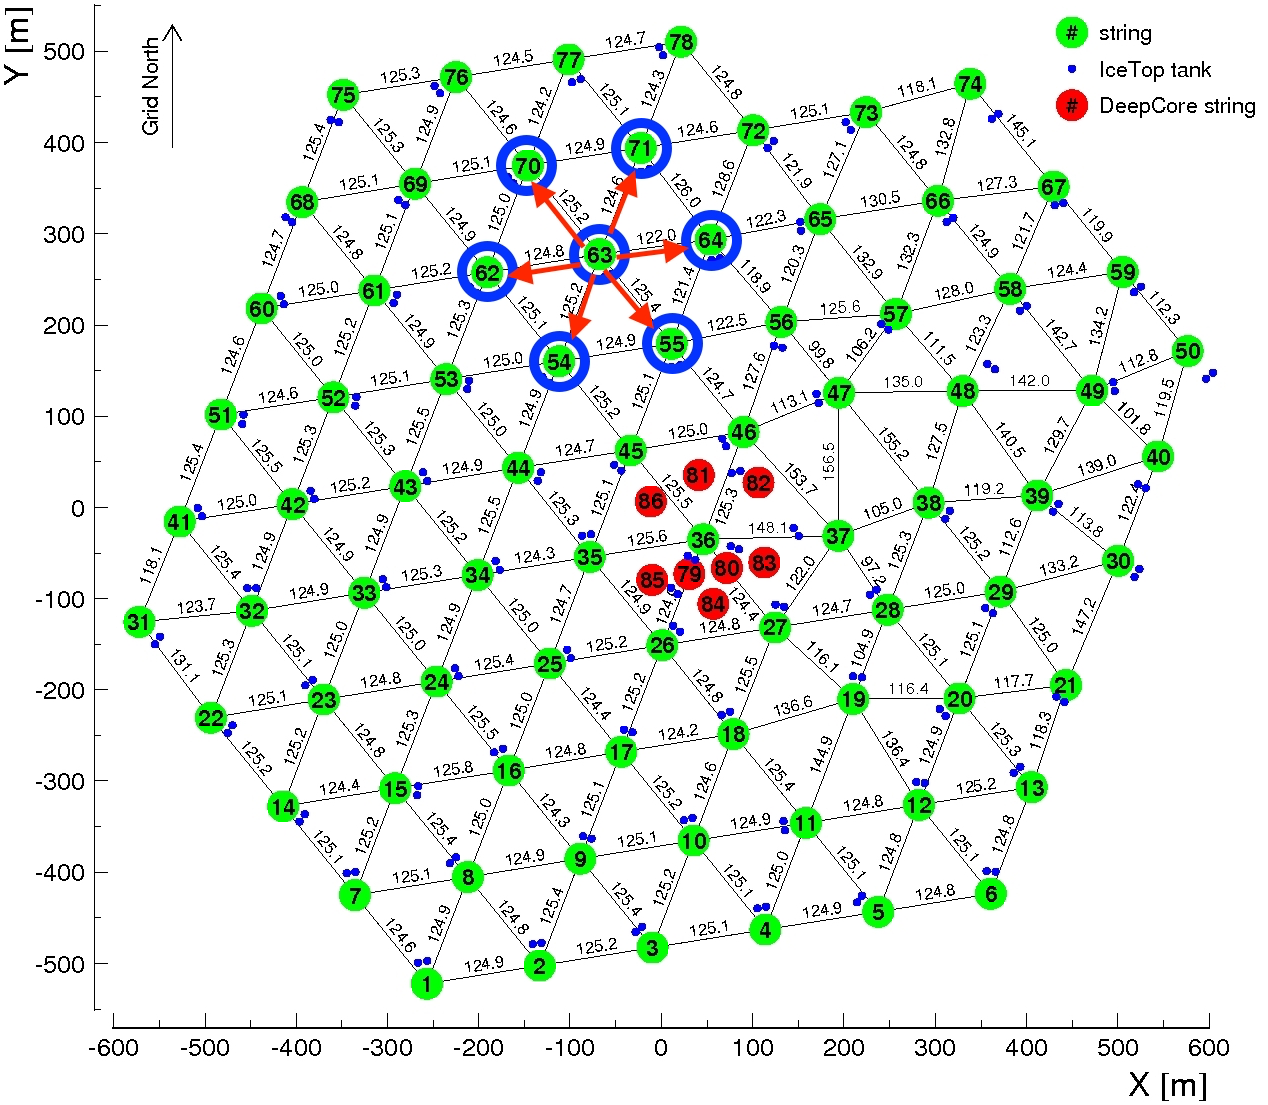
\includegraphics[width=.48\linewidth]{img/flasher-scenario}}
  \caption{Foo}
\end{figure}

- aim: adjust hole-ice parameters in simulation until the data curve is reproduced
- \docpar{This preliminary 7-string flasher study is documented in \issue{59}.}

- as seen in the figure, strings .. and .. are systematically reduced.
  - this might be due to cable shadows: #60
  - but also to sending dom not being cetered in its hole-ice column such that light is suppressed in this direction
  - out of scope
  - as an exmaple, fit only for receiving strings ...

- all-purpose flasher data set 2012
- source: path from 2018-03-21


- steamshovel figures: starting light, incoming at dom

- as a measure for comparing the simulation to the data,
- poisson likelihood is used
  - poisson likelihood, 2018-07-13
  - with weights, 2018-07-17, thorsten
  - gluesenkamp-3.pdf, S. 57

- contours figure

\begin{figure}[htbp]
  \smallerimage{flasher-contours-59}
  \caption{caption}
  \label{fig:label}
\end{figure}

- the contours show a valley where the simulated hole ice leads to good agreement of simulation and calibration data
- if the radius is too small or the scattering length is too large, the hole ice effect is too small and the amount of light arriving at the receiving doms is too high compared to the flasher data
- if the radius is too large or the scattering length is too small, the hole ice effect is too strong and the amount of light arriving at the receiving doms is too low compared to the flasher data

